\documentclass[11pt,a4paper]{article}
\usepackage[utf8]{inputenc}
\usepackage[czech]{babel}
%\usepackage{amsfonts}
%\usepackage{amsthm}
%\usepackage{amsmath}
%\usepackage{amssymb}
\usepackage[pdftex]{graphicx}
%\usepackage{enumerate}
%\usepackage{stmaryrd}
\usepackage{hyperref}
\usepackage{wasysym}

%\newtheorem{tvrz}{Tvrzení}
%\newtheorem{uloh}{Úloha}
%\newtheorem{lem}[tvrz]{Lemma}

\newcommand{\HRule}{\rule{\linewidth}{0.5mm}}
\newcommand{\cpp}{\textsc{C++}}
\newcommand{\mpp}{\textsc{Matrix++}}

\begin{document}

\begin{titlepage}
\begin{center}
% Upper part of the page

\includegraphics[viewport=180 50 100 100,scale=0.5]{./logo_mff.jpg}\\[1cm]    

\textsc{\LARGE Matematicko-fyzikální fakulta\\[0.1cm]
Univerzity Karlovy v Praze}\\[1.5cm]

\textsc{\Large Zápočtový program k NPRG041\\ ZS 2012/2013}\\[0.5cm]


% Title
\HRule \\[0.4cm]
{ \huge \bfseries Knihovna \mpp}\\[0.4cm]

\HRule \\[1.5cm]

% Author and supervisor
\begin{minipage}{0.4\textwidth}
\begin{flushleft} \large
\emph{Autor:}\\
Karel~\textsc{Ha}
\end{flushleft}
\end{minipage}
\begin{minipage}{0.4\textwidth}
\begin{flushright} \large
\emph{Cvičící:} \\
RNDr.~F.~\textsc{Zavoral},~Ph. D.
\end{flushright}
\end{minipage}

\vfill
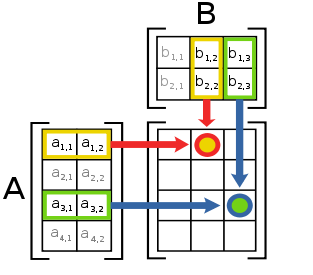
\includegraphics[viewport=140 15 150 65,scale=0.75]{./front.png}\\[1cm]    

% Bottom of the page
{\large \today}

\end{center}

\end{titlepage}

\thispagestyle{empty}

\begin{abstract}
Dokumentace k zápočtovému programu.
Práce je implementací ša\-blo\-no\-va\-né knihovny pro práci s maticemi
representované ve formě kontejnerů jazyka~\cpp.
\end{abstract}

\pagebreak

\thispagestyle{empty}
\tableofcontents

\pagebreak

\setcounter{page}{1}
\pagestyle{headings}

\part{Předmluva}

Text, jenž právě čtete, dokumentuje knihovnu \mpp.
Ta manipuluje s~matematickými maticemi formou kontejnerů programovacího jazyka
C++.
Konkrétně, pro zvolený datový typ a pro zadaný způsob manipulace s prvky
(neboli pro zadané \emph{těleso\/}, nad nímž chceme matici definovat) je skrze
šablony vygenerována jednotlivá třída.

Dále jsou implementovány základní maticové operace: sčítání, odčítání, násobení
skalárem, násobení dvou matic, transposice a další.

Mimojiné je zahrnuta podpora funkcí specifických pro jazyk \cpp: přetí\-že\-ní
operátorů $\ll$ a $\gg$ pro vstupně/výstupní operace; konstruktury a
destruktory kanonické formy; konversní operátory a konstruktory; členské
po\-lož\-ky a~metody splňující normu o~kontejnerech a~iterátorech
\cite{iso-norma}.

Nadto, jakožto praktická aplikace schopností tohoto rozhraní, byl implementován
QR rozklad a~QR algoritmus používáný pro výpočet vlastních čísel.

\pagebreak

\part{Programátorský manuál}
\section{Anotace}
Knihovna pro práci s grafy orientovanými a neorientovanými (a třeba také s
multigrafy nebo hypergrafy) --- definuje si nějaké rozumné uložení grafu
v~paměti (třeba pole vrcholů a seznamy hran z vrcholů vycházejících) a~nabízí
funkce pro běžné grafové operace (např.\ hledání nejkratší cesty, minimální
kostry, komponent souvislosti, transitivní redukce či uzávěru, topologické
třídění grafu). 

\section{Přesné zadání}
Implementace běžných operací s maticemi (sčítání, násobení, inverze,
determinant) použitím efektivních algoritmů. 
Matice bude representována ná\-sle\-du\-jí\-cí datovou strukturou:

\renewcommand{\labelitemi}{$\spadesuit$}

\begin{itemize}
\item \textbf{Pole vrcholů} obsahující informace o svých následovnících.
\item \textbf{Spoják následovníků} u každého vrcholu, obsahující navíc
informaci o váze (resp. ceně) hrany.
\end{itemize}

Dále bude nad digrafy možné provádět následující operace:

\renewcommand{\labelitemi}{$\clubsuit$}

\begin{itemize}
\item \textbf{Sym} orientující každou hranu digrafu {\sl do obou směrů\/}.
\item \textbf{Dijkstra} hledající vzdálenosti (tj.\ délky nejkratších cest) od
zadaného vrcholu ke všem ostatním vrcholům digrafu.
\item \textbf{Floyd-Warshall} hledající vzdálenosti mezi každými dvěma vrcholy
digrafu.
\item \textbf{Tarjan} hledající komponenty silné souvislosti za pomoci
Tarjanova algoritmu.
\item \textbf{TSort} hledající topologické uspořádání a v případě neexistence
výpis o přítomnosti cyklu v digrafu.%
\footnote{Což je ekvivalentní s neexistencí topologického uspořádání v digrafu.}
\item \textbf{Closure} hledající transitivní uzávěr digrafu.
\item \textbf{Reduction} hledající transitivní redukci digrafu.%
\footnote{Pozn. autora: Tato implementace zatím zvládá jen transitivní redukci
  v acyklických grafech.}
\end{itemize}

\section{Algoritmy a datové struktury}
\subsection{Použité datové struktury}
V této sekci si přiblížíme datové části použité v programu.

\begin{tabular}{ | c || r | l | p{4cm} | }
  \hline
  \textbf{Hlavní} & \textbf{Datový} & \textbf{Název} & \textbf{Popis} \\
  \textbf{struktura} & \textbf{typ položky} & \textbf{položky} & \\
  \hline \hline
  arc & unsigned int & index & \textit{index vrcholu, do něhož vede hrana} \\
  & double & weight & \textit{váha (potažmo cena) dané hrany} \\ 
  & arc * & next & \textit{ukazatel na další hranu (resp. dalšího následovníka)
    v~ pořadí} \\
  \hline \hline
  node & arc * & successors & \textit{spoják sousedů} \\
  \hline \hline
  graph & unsigned int & size & \textit{počet vrcholů} \\
  & unsigned int & order & \textit{počet hran} \\
  & node * & nodes & \textit{pole vrcholů} \\ 
  \hline \hline
  heap & unsigned int & regularity & \textit{max.\ počet potomků 1 uzlu v haldě} \\
  & int * & indices & \textit{pole s umístěním každého vrcholu grafu vzhledem
    haldě} \\
  & int * & heap\_arr & \textit{samotná halda s indexy náležejících vrcholů} \\
  & int & bottom & \textit{konec haldy} \\ 
  \hline \hline
  c\_bit & unsigned int : 1 & bit & \textit{bit na matici příznaků} \\
  \hline \hline
  llist\_node & unsigned int & val & \textit{hodnota uzlu spojáku} \\
  & llist\_node * & next & \textit{ukazatel na další uzel ve~spojáku} \\
  \hline \hline
  queue & llist\_node * & head & \textit{začátek fronty (odtud se odchází)} \\
  & llist\_node* & tail & \textit{konec fronty (sem se přichází)} \\
  \hline
\end{tabular}

Životně důležitou strukturou je {\tt graph}, v němž je vstupní graf uložen jako
seznam následovníků.

Na druhou stranu {\tt c\_bit} slouží pro jednoduché (neboli šetřící pamět,
poněvadž se jedná o pouhé samostatné bity) ukládání matic sousednosti.

{\sl Dijkstrův algoritmus\/} pro hledání vzdáleností využívá $k$-regulární
haldy, kde $k$ je určeno v položce {\tt regularity}.

Pro {\sl Tarjanův algoritmus\/} na hledání silně souvislých komponent je
využita zásobníková struktura {\tt queue}.

\subsection{Použité algoritmy}
V této sekci si popíšeme algoritmy použité pro operace nad grafy.
Jedná se {\sl de facto\/} o jádro {\tt GraphAlpha}, jež tvoří slavné algoritmy
velikánů informatiky jakými jsou např.\ {\sl Tarjan\/ {\rm či} Dijkstra\/}.
Půjde spíše o \uv{nošení dříví do lesa}, neboť tyto algoritmy jsou velmi známé
a dobře prozkoumané.

\subsubsection{Napojení knihovny na program}
Knihovna {\tt GraphAlpha} je psána v jazyku C a její integrování do programu je
velice jednoduché.
Soubory knihovny {\tt GraphAlpha.h} a {\tt GraphAlpha.c} stačí zkopírovat do
složky s programem využívající této knihovny a do programu vložit následující
řádek:

\begin{verbatim}
#include "GraphAlpha.h"
\end{verbatim}

To nalinkuje hlavičky funkcí a datové struktury knihovny.
Dál je nutné při kompilaci zkompilovat soubory knihovny a připojit je ke
kompilovanému programu.%
\footnote{Jako příklad tohoto může posloužit přiložený \tt Makefile}

\subsubsection{Funkce \tt symMtrx}

Funkce má následující hlavičku:

\begin{verbatim}
double** symMtrx(graph* p_gr);
\end{verbatim}

Ve stručnosti si popíšeme, co funkce dělá:

\renewcommand{\labelitemi}{$\sharp$}

\begin{itemize}
\item Převede representaci se seznamem následovníků na \uv{matici sousednosti},
  kde však místo $1$ a $0$ jsou váhy hran a hodnota {\tt DBL\_MAX}.%
  \footnote{pro vrcholy nespojené hranou.}
\item Porovnává po složkách hodnoty této matice a hodnoty její transposice%
\footnote{Jinak řečeno u každé dvojice vrcholů zkoumá tam i zpět.}
a, pokud jsou na obou místech platné hodnoty,%
\footnote{tedy existují hrany tam i zpět}
vezme se v absolutní hodnotě ta větší.
Je-li přítomna hrana jen jedním směrem, vytvoří se i identická hrana druhým
směrem.
\item Výsledek se vrací jako ukazatel na $2$-D pole.
\end{itemize}

Dále hlavní program {\tt main.c} zpracová toto pole tak, že ho za pomocí funkce
{\tt listConvert} převede na representaci se seznamem následovníků.
Ten se následovně zobrazí procedurou {\tt displayGraph} umístěné v {\tt main.c}.

\vskip .25cm

{\bf Časová složitost}
Převod na matici sice probere celý graf, ale vzhledem k nutnosti inicializace
matice a její následné projetí kvůli symetrisaci musí algoritmus vždy zpracovat celou matici.
Nechť ve zbytku textu $n$ značí počet vrcholů, $m$ počet hran, $T(n)$ časovou a
$S(n)$ paměťovou nárořnost.
Pak $T(n)\in\Theta(n^2)$

\vskip .25cm

{\bf Prostorová složitost}
Analogicky je vždy zapotřebí celá {\sl matice sousednosti\/}.
Tudíž podobně $S(n)\in\Theta(n^2)$

\subsubsection{Funkce \tt dijkstra}

Funkce má následující hlavičku:

\begin{verbatim}
double* Dijkstra (int v, graph* p_gr);
\end{verbatim}

Idea {\sl Dijkstrova algoritmu} je následující:

Představme si, že u každého vrcholu máme budík.
Na začátku jsou všechny nenastavené (tj.\ nastaveny na \uv{$\infty$}%
\footnote{zde řešeno pomocí \tt DBL\_MAX}),
až na zadaný výchozí vrchol, který je nastavený na $0$ (tj.\ zazvoní hned).

Dále algoritmus pracuje v cyklech.

Na začátku každého cyklu se probere vrchol, jemuž zazvoní budík nyní jako
první.
Jeho čas probuzení určí kýženou vzdálenost od startovního vrcholu.
Dále může tento vrchol tzv.\ {\sl zrelaxovat} hrany k sousedům, tedy
p ařena\-stavit jim časy probuzení, pokud by příslušné budíky za doby určené
vahami příslušných hran zazvonily dříve než mají aktuálně nastaveno.

Takto se pokračuje v cyklech dál, dokud stále nějaký budík tiká.

Je jasné, že {\sl Dijkstrův algoritmus} není nic jiného než-li obyčejná {\sl
diskrétní simulace\/}.%
\footnote{Z tohoto důvodu {\sl D. A.} zkolabuje na grafech se zápornými
  hranami, neb by se přes ně dalo vracet v čase a simulace by již nebyla
  simulací.}

\vskip .25cm

{\bf Časová složitost}
Klíčový je zde způsob výběru vrcholu s minimálním časem probuzení.
K tomu je zapotřebí vybrat vhodnou datovou strukturu, která dokáže rychle
provádět operaci {\sl Insert, Decrease\/ \rm a \sl ExtractMin\/}.

V řeči matematické, jsou-li $T_I$, $T_D$ a $T_E$ po řadě doby trvání operací
{\sl Insert, Decrease\/ {\rm a} ExtractMin}, pak časová složitost celého
algoritmu činí $T(n)\in\mathcal{O}(n \times (T_I + T_E) + m \times T_D)$.

Pro tento účel je jako stvořená tzv.\ {\sl halda\/} nebo ještě lépe její
zobecněná verse tzv.\ {\sl k-regulární haldy\/} s následujícími časy operací:

\renewcommand{\labelitemi}{$\diamond$}
\begin{itemize}
\item $T_I\in\mathcal{O}(\log_k n)$
\item $T_D\in\mathcal{O}(\log_k n)$
\item $T_E\in\mathcal{O}(k\log_k n)$
\end{itemize}

Po menších úpravách vyjde $T(n)\in\mathcal{O}( (kn + m) \log_k n )$.

Je očividné, že se zvětšujícím se $k$ logaritmus snižuje asymptotickou
složitost.
Zároveň se tím ale i zvyšuje multiplikativní konstanta.
Ovšem asymptoticky nám nebude vadit, pokud $k$ budeme zvyšovat až do takové
míry, kdy $kn = m$,%
\footnote{Dokonce stačí $kn\in\mathcal{O}(m)$}
neboť člen $m$ nám stále dokáže přebít člen $kn$.
Tedy stačí nastavit $k := \max\{2, \lfloor{m\over n}\rfloor\}$%
\footnote{Musí být $k\geq2$, aby se stále jednalo o haldu.}

Celkově vychází $T(n)\in\mathcal{O}(m \log_{m \over n} n) = \mathcal{O}({m
  \log n \over \log m - \log n})$

\vskip .25cm

{\bf Prostorová složitost}
Krom paměti pro uložení grafu ještě využíváme pole pro zaznamení vzdáleností a
$k$-regulární haldy, které však zaberou každý vrchol nejvýše jednou, takže
$S(n)\in\mathcal{O}(n)$, což je ovšem k nutnosti ukládat celý graf i s hranami
pořád asymptoticky {\sl okay\/}.
\subsubsection{Funkce \tt FloydWarshall}

Tato funkce má následující podobu:

\begin{verbatim}
double** FloydWarshall(graph* p_gr);
\end{verbatim}

Na tomto algoritmu je nádherně názorná síla {\sl dynamického programování\/}.
Označme si vrcholy libovolně indexy $1, 2, \dots n$.
Teď uvažme veličinu $D_{ij}^k$ jako délku nejkratší cesty z $i$ do $j$
využívající uvnitř pouze vrcholy $1, 2, \dots k$.

Nelze si nepovšimnout následujících pozorování:

$$D_{ij}^0 = \left\{ \begin{array}{ll}
  w(i, j) & \mbox{iff $(i, j)\in E(G)$}; \\
  \infty & \mbox{jinak}, \end{array} \right.$$

kde $w(i,j)$ označuje váhu hrany $ij$,

$$D_{ij}^n = d(i, j),$$

kde $d(i, j)$ označuje vzdálenost od $i$ do $j$, a nakonec důležitý rekursivní
vztah

$$D_{ij}^{k+1} = \min \{ D_{ij}^k, D_{i, k+1}^k + D_{k+1, i}^k \}.$$

Nyní přichází takový malý trik!
Platí zároveň i tyto 2 vztahy:

$$D_{i, k+1}^k = D_{i, k+1}^{k+1},$$
$$D_{k+1, i}^k = D_{k+1, i}^{k+1}.$$

To je z toho důvodu, že vrchol $k+1$ je krajní, tudíž je použit takjakotak a je
tedy zbytečné ho používat uprostřed cesty.%
\footnote{Tedy nadvakrát!!}
To nám ovšem značně zjednoduší práci i paměť, páč stačí použít jedinou matici.
Ač jsou v této matici smíchány v jediném cyklu hodnoty jak pro prvních $k$, tak
pro prvních $k+1$~vrcholů, můžeme si dovolit používat obě hodnoty, páč je to
jedno dle dvou předchozích pozorování.
Pro objasnění si lze algoritmus prohlédnout ve zdrojovém kódu.

\vskip .25cm

{\bf Časová složitost}
Pro celkově $n$ horních indexů vyplňujeme matici $n\times n$.
Složitost vychází $T(n)\in\Theta(n^3)$.

\vskip .25cm

{\bf Prostorová složitost}
Vždy si vystačíme s jedinou maticí $n\times n$.
Složitost je $S(n)\in\Theta(n^2)$.

\subsubsection{Funkce \tt Tarjan}

Tato funkce má tuto hlavičku:

\begin{verbatim}
void Tarjan(graph* p_gr);
\end{verbatim}

Popisovat {\sl Tarjanův algortimus\/} pro hledání {\sl silně souvislých
  komponent\/} je v jistém smyslu zbytečné---je již podrobně (a doufám si
  tvrdit, že i mnohem srozumitelněji) popsán na mnoha jiných místech.%
\footnote{Za všechny uveďme
  \url{http://en.wikipedia.org/wiki/Tarjan\%27s\_strongly\_connected\_components\_algorithm}}
Takže jen opravdu stručně:

Algoritmus je ve své podstatě modifikací {\sl DFS\/%
\footnote{\sl Depth-first search---\rm prohledávání do hloubky}
  algoritmu\/}.
Kromě hodnoty {\sl in\/}---času příchodu---řeší ještě tzv.\ hodnotu {\sl
  low\/}.
Ta je ve značné míře svázána s tzv.\ {\sl kořeny SSK.\/}%
\footnote{silně souvislých komponent}
To je vždy ten vrchol, jenž byl vzhledem ke~své {\sl SSK\/} navštíven jako
první%
\footnote{Tedy má ve své {\sl SSK\/} nejnižší hodnotu \sl in.}
a {\sl low\/} je jeho hodnota, která je stejná v celé příslušné {\sl SSK\/}.

Při průchodu grafem do hloubky se {\tt Tarjan} snaží minimalisovat hodnotu {\sl
  low\/} u každého vrcholu.
Dojde-li se do již navštíveného vrcholu,%
\footnote{Tedy šlo se po zpětné hraně.}
musí ležet v {\sl SSK\/} společné se svým předchůdcem a může mu tím pádem
snížit {\sl low\/}, neb onen následovník může být sám kořenem {\sl SSK\/}.

Dále se informace o {\sl low\/} propagují zpět při {\sl backtrace\/}, takže
každý vrchol pozná, zda je či není kořenem.%
\footnote{Ten má očividně \sl low(root) $==$ in(root)}
Pokud ano, okamžitě se ze zásobníku odeberou vrcholy s vyšším {\sl in\/},
poněvadž k těmto vrcholům lze dojít z kořene, a jelikož měli {\sl low\/} nižší
než {\sl in\/},%
\footnote{{\sl low\/} je nerostoucí funkce!}
sami nemůžou být {\sl kořenem\/}.

Navíc vrcholy nepřístupné z {\sl kořene} se nám zde neobjeví, páč k těm jsme
ani nemohli dojít aniž bychom nejprve neuzavřeli poslední {\sl SSK\/}.

\vskip .25cm

{\bf Časová složitost}
Jakožto modifikace {\sl DFS} má algoritmus náročnost $T(n)\in\Theta(n+m)$.
Problém by mohli činit testy navíc, které provádíme při ověření nenavštívenosti
vrcholů či jejich přítomnosti v zásobníku.
Toto vše lze však pomocí polí příznaků zvládat v konstantních časech, což se
nám asymptoticky schová do $\Theta$.

\vskip .25cm

{\bf Prostorová složitost}
Co je potřeba...
\renewcommand{\labelitemi}{$\nabla$}
\begin{itemize}
\item pole {\sl low\/}
\item pole {\sl in\/}
\item příznaková pole pro ověření navštívených vrcholů 
\item příznaková pole přítomnosti v zásobníku
\item zásobník pro vrcholy
\item zásobník pro rekursivní volání funkce {\sl DFS}
\end{itemize}

To vše postačuje ve velikosti odpovídající počtu vrcholů, ergo paměti je třeba
$S(n)\in\Theta(n)$.

%TODO
\subsubsection{Funkce \tt TSort}

Tato funkce má takovouto hlavičku:

\begin{verbatim}
int TSort(graph* p_gr, int* seq);
\end{verbatim}

Principem tohoto algoritmu je postupné odtrhávání {\sl výtoků\/}.%
\footnote{vrcholů, do nichž nevedou žádné hrany}
Pokud by totiž vedla hrana z aktuálního výtoku do nějakého již odtrženého
vrcholu, ten by pak v době svého odtržení nemohl sám býti výtokem, poněvadž do
něj vede hrana z původního uvažovaného výtoku.
To je ovšem spor \lightning

Nejprve se průchodem všemi vrcholy určí {\sl vstupní stupně\/}%
\footnote{počet hran končících ve vrcholu}
vrcholů.
Poté umístíme do fronty všechny vrcholy s nulovým vstupním stupněm%
\footnote{tj. \sl výtoky}
a ty budeme postupně zařazovat do {\sl topologického uspořádání\/}.
U každého vrcholu budeme navíc jeho sousedům {\sl dekrementovat\/}%
\footnote{snižovat o 1}
vstupní stupně v nově vznikajícím grafu.

Dojdou-li všechny výtoky ještě před koncem, graf žádné {\sl topologické
uspořádání\/} nemá a není tudíž acyklický. Právě toto se vypíše.

\vskip .35cm

{\bf Časová složitost}
Průchod grafem pro zjištení {\sl vstupních stupňů\/} zabere (jako každý průchod
grafem) $\Theta(n + m)$ času.

Každý vrchol se odtrhne nejvýše jednou a přes každou hranu se i nanejvýš jednou
dekrementuje.

To činí $T(n)\in\Theta(n + m)$.

\vfil\eject

{\bf Prostorová složitost}
Vždy pracujeme s datovými entitami pojímající informaci ke každému z vrcholu.
K tomu ještě zásobník pro výtoky, který však maximálně bude pojímat všechny
vrcholy.

{\sl Sumo sumárum $S(n)\in\Theta(n)$.}

\subsubsection{Funkce \tt transitiveClosure}

Funkce s následující hlavičkou:

\begin{verbatim}
c_bit** transitiveClosure(graph* p_gr);
\end{verbatim}

Uzávěr lze získat mnoha způsoby.
Je třeba jen spojit hranou vrcholy, mezi kterými existuje cesta.

Jedním způsobem je pustit na graf funkci {\tt FloydWarshall} a spojit
hranou vrcholy, které mají vzdálenost menší než $\infty$.

Ještě jednodnušším způsobem jest menší úprava aktualizačního přiřazování uvnitř
\uv{trojcyklu}:

$$e_{ij}^{k+1} = e_{ij}^k \vee (e_{i, k+1}^k \wedge e_{k+1, i}^k)$$

kde $e_{ij}^k$ značí příznak přítomnost $i \rightarrow j$ cesty využívající
prvních $k$ vrcholů. 

\vskip .25cm

{\bf Časová složitost}
Jedná se jen o upravený {\sl Floyd-Warshallův algoritmus} $\Rightarrow
T(n)\in\Theta(n^3)$.

\vskip .25cm

{\bf Prostorová složitost}
Stále jen upravený {\sl Floyd-Warshallův algoritmus} $\Rightarrow
S(n)\in\Theta(n^2)$.

\subsubsection{Funkce \tt transitiveReduction}

Funkce s následující hlavičkou:

\begin{verbatim}
c_bit** transitiveReduction(graph* p_gr);
\end{verbatim}

Algoritmus využívá následujícího pozorování---pro acyklický graf $R$ platí

$$R^- = R \setminus (R \circ R^+), $$

kde $R^-$, $R^+$ značí po řadě {\sl transitivní redukci\/} a {\sl transitivní
  uzávěr\/}%
\footnote{bez smyček---hran do stejného vrcholu}
uvažo\-va\-ného grafu $R$.

To funguje z následujícího důvodu---$(R \circ R^+)$ jsou všechny dvojice
vrcholů, mezi kterými vede cesta s alespoň jedním mezivrcholem.
Po odebrání těchto \uv{přebytečných hran} zbydou jen dvojice vrcholů
bezprostředně násle\-dující po sobě.

To by však zkolabovalo u vrcholu \uv{napojeného} na cyklus%
\footnote{Příklad takovéhoto grafu lze nalézt v \tt testing/reduction\_cyclic.in}
v grafu---odebrala by se totiž i hrana mezi vrcholem a cyklem, již potřebujeme.

\vskip .25cm

{\bf Časová složitost}
Potřebujeme nejprve získat {\sl transitivní uzávěr} za pomoci funkce {\tt
  transitiveClosure}.
Dále postupujeme dle výše uvedeného vzorce.

Zřejmě největší obtíže nám bude činit výpočet operace složení relací.
Uvažme ale nejhorší případ---tedy úplný graf $K_n$.
Jeho uzávěr má $\mathcal{O}(n^2)$ hran, každá lze složit s libovolným dalším z
$\mathcal{O}(n)$ vrcholů.
Tedy skládání se zvládne v čase $\mathcal{O}(n^3)$.

Množinový rozdíl už je {\sl triviální} záležitost na $\Theta(n^2)$ času.

Celkově tedy $T(n)\in\Theta(n^3)$.

\vskip .25cm

{\bf Prostorová složitost}
Pro vzorec využíváme jen 3 matice.
Takže pro paměť platí $S(n)\in\Theta(n^2)$.

\subsubsection{Další funkce $\dots$}
Mezi další funkce náleží takové \uv{vychytávky} jako

\renewcommand{\labelitemi}{$\bowtie$}
\begin{itemize}
\item převod mezi $2$ používanými representacemi grafu
\item zobrazení grafu
\item vyčištění obrazovky
\item ukončení programu
\end{itemize}

U těchto funkcí si autor dovoluje vynechat pasáže o časových a prostorových
náročnostech, páč, jak se čtenář ze zdrojového textu sám přesvědčí, se jedná o
pouhé triviality {\tt :-)}

\pagebreak

\part{Uživatelský manuál}
Pro účely názorné demonstrace knihovny {\sl GraphAlpha} byl sepsán obslužný
program umístěný v souboru \verb=main.c=.
Ten je zcela separován od knihovních funkcí, tudíž operace nad grafy lze
libovolně kombinovat (např.\ vytvořit neorientovanou versi transitivní redukce)
či využívat je jakožto součást jiných programů.

\section{Menu}
Při spuštění obsluhy nás uvítá zpráva o aktuální versi ovládacího programu:

\vskip .25cm
{\tt
\noindent Welcome to GraphAlpha v1.3! \\
\noindent This is a demonstration program of GraphAlpha library.
}
\vskip .25cm

\noindent Následuje dotaz na parametry vstupního grafu:
\vskip .25cm
{\tt
\noindent Enter count of nodes: {\bf 3} \\
\noindent Enter count of arcs: {\bf 2}
}
\vskip .25cm

Program se poté zeptá na detaily jednotlivých hran:

\begin{verbatim}
1. node
 From:  
 To:  
 Weight:
2. node
 From:  
 To:
 Weight: 
\end{verbatim}

Jedná se o následující údaje:
\renewcommand{\labelitemi}{$\propto$}
\begin{itemize}
\item {\sl From:\/} výstupní vrchol, ze kterého zadávaná hrana vede
\item {\sl To:\/} vstupní vrchol, do kterého zadávaná hrana vede
\item {\sl Weight:\/} váha (popř. cena), zadávané hrany
\end{itemize}

Každá hrana obsahuje návěští s pořadovým číslem zadávané hrany.

Nakonec nabídne aplikace nabídku poskytovaných příkazů.
Tyto lze spatřit na následující stránce $\dots$

\vfill\eject

\begin{verbatim}
---------------------------------------------------------------
Choose option (enter the part in brackets)
(S)ym            - symmetrization
(D)ijkstra       - shortest path between node & other nodes
(F)loyd-Warshall - shortest path between every 2 nodes
tar(J)an         - strongly connected components
(T)sort          - topological ordering
(C)losure        - transitive closure
(R)eduction      - transitive reduction
l(I)st-convert   - from adjacency matrix to list of successors
(M)atrix-convert - from list of successors to adjacency matrix
c(L)ear          - clear screen (only for in *nix like OS) 
Displa(Y)        - display the graph 
(H)elp           - display this menu:) 
(Q)uit           - quit the program 
---------------------------------------------------------------
>>
\end{verbatim}

Jak vidno, tuto nabídku lze kdykolit znova vyvolat pomocí
příkazu {\tt h}:%
\footnote{Příkazy lze zadávat velkými i malými písmeny abecedy.
Dokonce ani nevadí, když jsou za prvním písmenem další znaky, ty se až do konce
  řádku ignorují.}

\begin{verbatim}
>> h 
\end{verbatim}

\section{Vstup a příkazy programu}
\subsection{Sym}
Příkaz, jenž \uv{zorientuje každou hranu na obě strany}, dokáže i zajistit
převod orientovaného grafu na neorientovaný.

\begin{verbatim}
>> s
List of successor representation:
1. node -> 3(3.140000)
3. node -> 1(3.140000)
Matrix representation:
----    ----    3.14
----    ----    ----
3.14    ----    ----
\end{verbatim}

{\noindent \sl Pozn.~Vstup z \tt testing/sym2.in}

\subsection{Dijkstra}
Příkaz spuštění {\sl Dijkstrova algoritmu\/} ze zadaného vrcholu.

\begin{verbatim}
>> d
Enter starting node of graph: 1
From 1.node to all nodes respectively:
0.000000 7.000000 9.000000 20.000000 20.000000 11.000000 
\end{verbatim}

{\noindent \sl Pozn.~Vstup z \tt testing/dijkstra2.in}

\subsection{Floyd-Warshall}
Příkaz spuštění {\sl Floyd-Warshallova algoritmu\/}.%
\footnote{Mimochodem tento algoritmus je použit pro vytvoření grafu
transitivního uzávěru v representaci se seznamem následovníků.
Autor tak učinil z dvou prostých důvodů: zaprvé Floyd-Warshall podává lepší
informaci o vahách mezi vrcholy jakožto jejich vzdálenosti; zadruhé algoritmus
transitivního uzávěru je jen upravená verse Floyd-Warshallova algoritmu \sl :-)}


\begin{verbatim}
>> f
List of successor representation (i.e., transitive closure):
1. node -> 4(3.600000) 2(1.200000) 1(1.100000)
2. node -> 4(2.400000)
3. node -> 4(6.700000) 2(4.300000) 1(3.100000)
Matrix representation:
1.10    1.20    ----    3.60
----    0.00    ----    2.40
3.10    4.30    0.00    6.70
----    ----    ----    0.00
\end{verbatim}

{\noindent \sl Pozn.~Vstup z \tt testing/floyd\_warshall.in}

\subsection{Tarjan}
Příkaz spuštění {\sl Tarjanova algoritmu\/}.%
\footnote{Počínaje od vrcholu s indexem 1, neb hlavní procedura zkoumá
  nezpracované vrcholy v rostoucím pořadí indexů.}%
\footnote{Tarjanův algoritmus zároveň určuje reversní topologické uspořádání
  grafu komponent zadaného grafu.}

\begin{verbatim}
>> j
( 7 6 )
( 8 4 3 )
( 5 2 1 )
\end{verbatim}

{\noindent \sl Pozn.~Vstup z \tt testing/scc2.in}

\subsection{TSort}
Příkaz spuštění algoritmu pro nalezení {\sl topologického uspořádání\/}.%
\footnote{V případě neexistence takového uspořádání (nastane právě v grafech s
  cykly) se vypíše \tt NOT AN ACYCLIC GRAPH!}

\begin{verbatim}
>> t
Topological ordering: 1 4 2 3 5
\end{verbatim}

{\noindent \sl Pozn.~Vstup z \tt testing/tsort.in}

\subsection{Closure}
Příkaz spuštění algoritmu pro vytvoření {\sl transitivního uzávěru\/}.%
\footnote{Zde použitá implementace funkce vrací matici sousednosti nalezeného
  uzávěru.
Ovšem knihovna poskytuje funkci {\tt listConvertBit}, jež matici dokáže převést
  na representaci se seznamem následovníků.
To je náležitě využito v {\tt main.c} pro zobrazení obou možných representací,
  jak si lze prohlédnout v přiloženém výstupu.}

\begin{verbatim}
>> c
List of successor representation:
1. node -> 5(1.000000) 4(1.000000) 3(1.000000) 2(1.000000) 1(1.000000)
2. node -> 5(1.000000) 3(1.000000) 2(1.000000)
3. node -> 5(1.000000) 3(1.000000)
4. node -> 5(1.000000) 4(1.000000) 3(1.000000)
5. node -> 5(1.000000)
Matrix representation:
1 1 1 1 1 
0 1 1 0 1 
0 0 1 0 1 
0 0 1 1 1 
0 0 0 0 1 
\end{verbatim}

{\noindent \sl Pozn.~Vstup z \tt testing/closure.in}

\subsection{Reduction}
Příkaz spuštění algoritmu pro vytvoření {\sl transitivního redukce.
\vskip .45cm
Pozn.~Tato implementace zvládá nalézt redukci {\bf pouze} v acyklických grafech.
Autor z důvodů časové tísně a značné vyspělosti obecného algoritmu nebyl
schopen vyřešit případ pro grafy s cykly a slibuje, že se do přístě napraví
\sl :-)}
\vskip .45cm

Výstup toho příkazu je k nalezení na další stránce $\dots$

\vfil\eject

\begin{verbatim}
>> r
List of successor representation:
1. node -> 4(1.000000) 2(1.000000)
2. node -> 3(1.000000)
3. node -> 5(1.000000)
4. node -> 3(1.000000)
Matrix representation:
0 1 0 1 0 
0 0 1 0 0 
0 0 0 0 1 
0 0 1 0 0 
0 0 0 0 0 
\end{verbatim}

{\noindent \sl Pozn.~Vstup z \tt testing/reduction2.in}

\begin{verbatim}
>> r
Warning! Given graph is NOT acyclic.
The result of transitive reduction is ungranted!
List of successor representation:
1. node -> 2(1.000000)
2. node -> 3(1.000000)
3. node -> 1(1.000000)
4. node -> 5(1.000000)
5. node -> 6(1.000000)
6. node -> 4(1.000000)
Matrix representation:
0 1 0 0 0 0 
0 0 1 0 0 0 
1 0 0 0 0 0 
0 0 0 0 1 0 
0 0 0 0 0 1 
0 0 0 1 0 0 
\end{verbatim}

{\noindent \sl Pozn.~Vstup z \tt testing/reduction\_cyclic.in}

\subsection{List-convert}
Příkaz spuštění pro převod {\sl maticové \rm representace na representaci se
  \sl seznamem následovníků\/}.%
\footnote{Příkaz dokáže fungovat obecně.
Pro účely jednoduchosti však {\sl main.c} využívá funkci tak, že seznam
  následovníků nejprve převede na matici a ta se pomocí {\sl list-convert}
  převede zpět.
Samozřejmě je list-convert využit ještě u funkcí vracející maticové
  representací jakými jsou například {\tt closure\/ {\rm či} reduction\/}.
}
\vfil\eject
\begin{verbatim}
>> i
Converting the already matrix-converted graph
  to list-of-sucessors representation...
1. node -> 4(0.200000) 3(0.600000) 2(0.200000)
2. node -> 3(0.300000)
3. node -> 5(0.500000)
4. node -> 5(0.800000) 3(0.200000)
\end{verbatim}

{\noindent \sl Pozn.~Vstup z \tt testing/list\_convert.in}

\subsection{Matrix-convert}
Příkaz spuštění pro převod se {\sl seznamem následovníků \rm representace na
  representaci \sl maticovou\/}.%
\footnote{Příkaz dokáže fungovat obecně.
Pro účely jednoduchosti však {\tt main.c} využívá funkci tak, že seznam
  následovníků nejprve převede na matici a ta se pomocí {\tt list-convert}
  převede zpět.
Samozřejmě je list-convert využit ještě u funkcí vracející maticové
  representací jakými jsou například {\tt closure či \tt reduction\/}.
}

\begin{verbatim}
>> m

----    0.20    0.60    0.20    ----
----    ----    0.30    ----    ----
----    ----    ----    ----    0.50
----    ----    0.20    ----    0.80
----    ----    ----    ----    ----
\end{verbatim}

{\noindent \sl Pozn.~Vstup z \tt testing/matrix\_convert.in}

\subsection{Display}
Příkaz pro zobrazení grafu v representaci se seznamem následovníků.

\noindent {\bf Formát:}

\noindent {\sl $<$index výchozího uzlu$>$\tt.node -> \sl $<$index příchozího
  uzlu$>$\tt (\sl$<$váha$>$\tt)}

\begin{verbatim}
>> y
1. node -> 4(0.200000) 3(0.600000) 2(0.200000)
2. node -> 3(0.300000)
3. node -> 5(0.500000)
4. node -> 5(0.800000) 3(0.200000)
\end{verbatim}

\subsection{Clear}
Příkaz na vyčištění obrazovky (v abstraktním slova smyslu, samozřejmě, jinak
použijte suchý hadřík či látku {\tt :-)}
Funguje převážně na systémech *nixového typu, páč využívá systémové procedury
\verb=clear=.

\begin{verbatim}
>> l
\end{verbatim}

\subsection{Quit}
A tady končí naše cesta...

\begin{verbatim}
>> q
Bye bye...
\end{verbatim}

\pagebreak

\part{Závěr}

Autor musí podotknout, že se nabízí nemalé množství prostoru pro vylepšení:
\begin{enumerate}
  \item {\bf Násobení matic\/} přímo podle definice není nejefektivnější.
    Lze vylepšit přepsáním funkce
\begin{verbatim}template<typename T>
Matrix<T> operator*(const Matrix<T> &, const Matrix<T> &);\end{verbatim}
    např. pomocí \emph{Strassenova algoritmu\/}.
\end{enumerate}

\pagebreak

\begin{thebibliography}{9}

\bibitem{iso-norma}
Norma \textsc{ISO/IEC N3290} programovacího jazyka \cpp.

\end{thebibliography}

\end{document}
